\section{Static Program Slicing for
Swift}\label{static-program-slicing-for-swift}

Jared Khan, St John's College

\textbf{Originator:} Dr S Kell

\textbf{Project Supervisor:} Dr S Kell

\textbf{Director of Studies:} Dr R Mullins

\textbf{Project Overseers:} Dr M Kuhn, Prof P Sewell

\subsection{Introduction}\label{introduction}

\providecommand{\tightlist}{%
  \setlength{\itemsep}{0pt}\setlength{\parskip}{0pt}}

Mark Weiser introduced the idea of program slicing in his 1989 thesis
{[}1{]}. Program slicing is the task of, given a slicing criterion
formed of a set of variables and a location in a source file, finding
the executable subset of instructions that can possibly affect the value
of any of those variables at that location.

The following example (taken from Frank Tip's 1994 survey of slicing
techniques {[}2{]}) demonstrates a short program and its slice with
respect to the criterion: (\texttt{sum}, line 13)

\begin{verbatim}
let n = readInt()
var sum = 0
var product = 1

var i = 1
while i < n {
    sum = sum + i
    product = product * i
    i = i + 1
}

print(product)
print(sum)
\end{verbatim}

\begin{verbatim}
let n = readInt()
var sum = 0


var i = 1
while i < n {
    sum = sum + i

    i = i + 1
}


print(sum)
\end{verbatim}

Weiser argues {[}6{]} that programmers use slicing instinctively in
their heads when trying to understand existing code and describes
techniques for automating the generation of these slices.

Uses for program slicing include:

\begin{itemize}
\tightlist
\item
  Debugging. For seeing the sequence of statements that led to the
  current state
\item
  Refactoring. e.g.~For extracting useful, narrower functionality from
  an existing function
\item
  Program Differencing (determining the set of changes between an old
  and a new version of a program).
\end{itemize}

An important distinction to make is that between static and dynamic
slicing. A \emph{static} slice is one which includes all lines that
could possibly affect the values at the slicing criterion in some
execution of the program. A \emph{dynamic} slice is one which uses
information about the current execution.

\begin{verbatim}
let y: Int
if x == 1 {
    y = 1
} else {
    y = 2
}
print(y)
\end{verbatim}

In this example, given the criterion (\texttt{y}, line 7), a static
slicer could not reduce this program. A dynamic slicer running in a
specific instance where execution has reached line 7 and \texttt{x} was
equal to 2 would be able to produce the following slice:

\begin{verbatim}
let y: Int



    y = 2

print(y)
\end{verbatim}

This is useful in a debugging setting.

For the purposes of this project I will focus on static slicing.

In this project I focus on executable slices. That is, the resulting
slices are, in themselves, executable Swift programs. The challenge that
this poses is that as well as the lines of the program that contribute
to the values at the slicing criterion, we also need to keep other lines
that allow the program to run. This is relevant only when slicing
programs with multiple procedures, as Tip {[}2{]} discusses. For a
minimal implementation, my slicer will initially deal with single
procedures and will leave multi-procedural slicing as an extension.

The Swift programming language is an increasingly popular high-level
language that compiles to native code via LLVM (Low Level Virtual
Machine) bitcode. Static slicers exist for LLVM bitcode {[}3{]}{[}4{]}
but no prominent slicer exists for Swift. The benefits of program
slicing are best exploited at the high-level. This project aims to
implement a static slicer for a significant subset of the Swift language
and compare the precision, that is the lack of irrelevant statements, of
the slices produced by slicing Swift source and compiling the results to
LLVM and compiling the Swift source to LLVM and then slicing the
results.

\subsection{Starting Point}\label{starting-point}

Frank Tip provides a survey {[}2{]} of the prominent slicing algorithms
in his paper ``A Survey of Program Slicing Techniques''. This provides a
good starting point for choosing a good algorithm for the slicing of
Swift. Static slicers have been successfully implemented for (subsets
of) other high-level languages.

The Swift compiler is an open source project. Part of this project is a
library called SourceKit, intended to help IDEs provide Swift language
support. This provides structural and syntactic information of source
programs towards this end. Since the parsing of Swift programs is not
directly relevant to the subject matter here, the goal will be to use as
much existing infrastructure as possible for my implementation. Third
party wrappers exist for the SourceKit library for better ergonomics and
use within Swift itself.

Though the choice of an appropriate algorithm is in itself an important
part of this project and is yet to be done, the infrastructure required
to implement these algorithms invariably involves the following:

\begin{enumerate}
\def\labelenumi{\arabic{enumi}.}
\tightlist
\item
  Identification of variable definition statements
\item
  Identification of variable references
\item
  Identification of branch statements
\item
  Identification of the variables that a condition expression relies
  upon
\item
  Identification of the statements that rely upon given branches
\end{enumerate}

SourceKit provides insight into all the above. Some notable challenges
that remain include:

\begin{enumerate}
\def\labelenumi{\arabic{enumi}.}
\tightlist
\item
  Correct handling of variable shadowing
\item
  Handling of early exits of functions (e.g.~from early \texttt{return}
  statements)
\end{enumerate}

\subsection{Description of the work}\label{description-of-the-work}

I will implement a static slicer for Swift that should aim for precision
with a lesser concern for performance (since the intention is for this
to be used as a static tool).

I will write a small set of single-procedure test cases that cover the
Swift language constructs that I aim to support. Depending on the subset
of the language I chose to support upon further investigation, I will
also select some segments of open source projects for use as test cases.
I will select slicing criteria for these test cases and slice these by
hand. I will then build a small program that will check that two Swift
programs are structurally identical. These things together provide a
test suite for checking correctness of my slicer.

I will adapt existing LLVM slicers {[}3{]}{[}4{]} for use with compiled
Swift programs. This only involves ensuring that I have a slicer that
can perform on a compatible LLVM bitcode version.

I will optionally build a tool to translate slicing criteria for Swift
source files to their corresponding criteria in the LLVM bitcode. This
will utilise the existing DWARF debugging information provided by Swift.
It may be that, upon investigation, this proves too much work to
automate and I will use manually translated slicing criteria.

I will test the code reduction achieved by each of the two routes (see
figure below) for various slicing criteria.

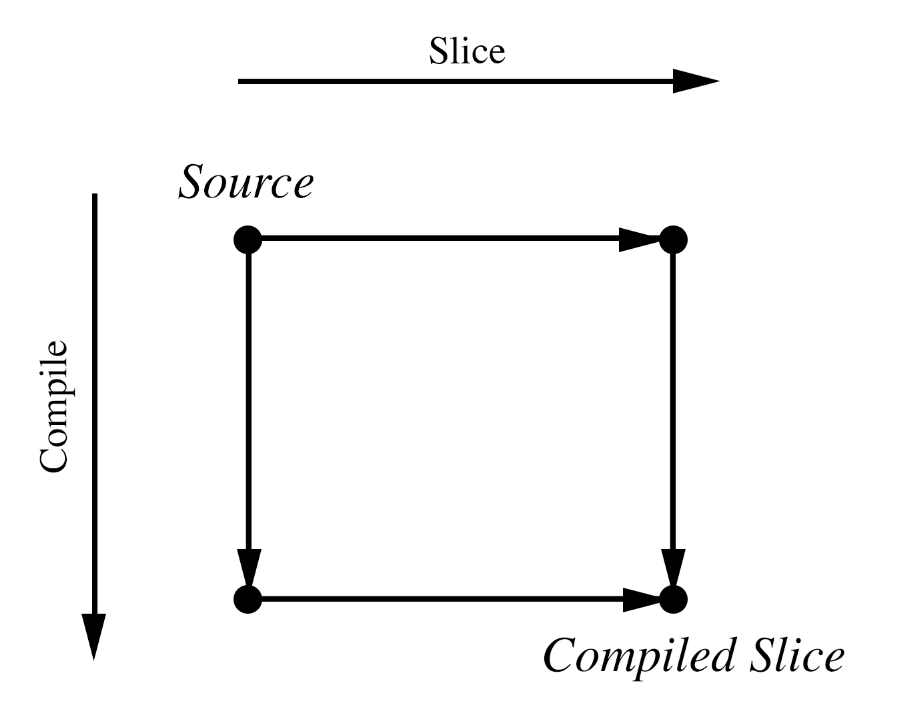
\includegraphics{SliceCompile.png} \textbf{Figure} Two routes from a
Swift source file to a sliced LLVM bitcode file: Compile to LLVM bitcode
then slice LLVM, Slice Swift then compile to LLVM bitcode. This allows a
direct quantitative comparison of my slicer and existing slicers.

I aim to show that my slicer is \emph{correct} and provides a reduction
in code comparable to that of compiling to LLVM and then slicing.

It will be unrealistic to expect to cater to \emph{all} of Swift in my
slicer. It is idiomatic in Swift to use value types (\texttt{enum}s,
\texttt{struct}s, \texttt{tuple}s) over reference types
(\texttt{class}es) to avoid the creation of shared mutable state. The
subset of Swift considered in this project in particular \emph{excludes}
reference types, higher-order functions, unstructured control flow
(\texttt{break}, \texttt{fallthrough}, \texttt{continue},
\texttt{throw}), labeled statements and compiler control statements.

\subsection{Success Criteria}\label{success-criteria}

Qualitative:

\begin{itemize}
\tightlist
\item
  Correctness of the slices in my static slicer (as verified by the
  devised test suite)
\item
  `Reasonable performance' (i.e. \textless{} 5 seconds to generate
  slices for a 1000 line program)
\end{itemize}

Quantitative:

\begin{itemize}
\tightlist
\item
  For equivalent slicing criteria, slicing at least half as much as the
  low level slicer achieves. (Since the compiled LLVM bitcode has finer
  grain instructions, I would expect the slicing of the bitcode to yield
  a greater reduction).
\end{itemize}

\subsection{Possible Extensions}\label{possible-extensions}

\begin{enumerate}
\def\labelenumi{\arabic{enumi}.}
\item
  Techniques exist for the slicing of multi-procedural programs. Time
  permitting, I will investigate these techniques for implementation in
  my slicer.
\item
  Techniques exist for the handling of unstructured control flow in
  program slicing. Time permitting, I will investigate these techniques
  for implementation in my slicer.
\item
  Techniques exist for the handling of reference types in program
  slicing. Time permitting, I will investigate these techniques for
  implementation in my slicer.
\item
  Ott and Beiman {[}5{]} describe a method for objectively defining the
  `cohesion' of a program based on static slices. Time permitting, I
  will implement their concept using my slicer and evaluate prominent
  open source projects before and after commits that claim to `refactor'
  to assess whether this metric is meaningful in practice.
\end{enumerate}

\subsection{Timetable and milestones}\label{timetable-and-milestones}

\begin{enumerate}
\def\labelenumi{\arabic{enumi}.}
\tightlist
\item
  \textbf{Michaelmas weeks 3--4}

  \begin{itemize}
  \tightlist
  \item
    Read Tip's Survey {[}2{]}
  \item
    (Time permitting) Read Ott and Beiman {[}5{]}
  \item
    (Time permitting) Investigation for extensions 1, 2, and/or 3
  \item
    Identify appropriate slicing techniques for precise static slicing
    of Swift
  \item
    Assess the amount of work required for successful use of existing
    LLVM slicers
  \item
    Identify the subset of the Swift grammar that I will initially
    support
  \end{itemize}
\item
  \textbf{Michaelmas weeks 5--6}

  \begin{itemize}
  \tightlist
  \item
    Write the test case programs
  \item
    (Time permitting) write test case programs for extensions 1, 2,
    and/or 3
  \item
    Identify the necessary Swift program representation required by the
    chosen slicing algorithm
  \item
    Implement data structures for this representation
  \item
    Create the representation of each of the test case programs by hand
    as test cases
  \item
    Implement the generation of the program representation
  \item
    \emph{Milestone:} The representation test suite passes (15 Nov)
  \end{itemize}
\item
  \textbf{Michaelmas weeks 7--8}

  \begin{itemize}
  \tightlist
  \item
    Write the program similarity checker
  \item
    Implement the slicing algorithm using the program representation
  \item
    (Time permitting) Extend the slicing algorithm with extensions 1, 2,
    and/or 3
  \item
    \emph{Milestone:} The slicing test suite passes (27 Nov)
  \end{itemize}
\item
  \textbf{Michaelmas vacation}

  \begin{itemize}
  \tightlist
  \item
    Build tool for translating slicing criteria from Swift to LLVM
    bitcode
  \item
    Write a small test suite for this
  \item
    \emph{Milestone}: (Optional) The criterion translator test suite
    passes (14 Dec)
  \item
    Slower pace over the break
  \end{itemize}
\item
  \textbf{Lent weeks 0--2}

  \begin{itemize}
  \tightlist
  \item
    Write progress report
  \item
    Write program to compare the reduction from the two slicing routes
  \end{itemize}
\item
  \textbf{Lent weeks 3--5}

  \begin{itemize}
  \tightlist
  \item
    Run experiments on test programs
  \item
    (Time permitting) Extension 4
  \item
    \emph{Milestone:} Have test results of the precision of my slicer vs
    that of LLVM slicers (14 Feb)
  \end{itemize}
\item
  \textbf{Lent weeks 6--8}

  \begin{itemize}
  \tightlist
  \item
    Dissertation outline and main chapters
  \end{itemize}
\item
  \textbf{Easter vacation:}

  \begin{itemize}
  \tightlist
  \item
    Complete first draft of dissertation and submit for review by
    supervisor
  \item
    \emph{Milestone:} Draft dissertation submitted (19 April)
  \item
    (Time permitting) Extension 4
  \end{itemize}
\item
  \textbf{Easter weeks 0--2:}

  \begin{itemize}
  \tightlist
  \item
    Responding to dissertation feedback
  \item
    Further evaluation and complete dissertation
  \item
    Proof reading and submission
  \item
    \emph{Milestone:} Dissertation submission (9 May) (Note due 18 May)
  \end{itemize}
\end{enumerate}

\subsection{Works Cited}\label{works-cited}

\noindent
{[}1{]}\\
Mark Weiser\\
Program slices: formal, psychological, and practical investigations of
an automatic program abstraction method\\
University of Michigan Ann Arbor, MI, USA\\
1979
\\
\\
\noindent
{[}2{]}\\
Frank Tip\\
A Survey of Program Slicing Techniques\\
CWI (Centre for Mathematics and Computer Science) Amsterdam, The
Netherlands, The Netherlands\\
1994
\\
\\
\noindent
{[}3{]}\\
Marek Chalupa\\
dg\\
https://github.com/mchalupa/dg\\
2017
\\
\\
\noindent
{[}4{]}\\
Jiri Slaby\\
https://github.com/jirislaby/LLVMSlicer\\
2015
\\
\\
\noindent
{[}5{]}\\
Ott and Bieman\\
Program Slices as an Abstraction for Cohesion Measurement\\
Information and Software Technology\\
1998
\\
\\
\noindent
{[}6{]}\\
Mark Weiser\\
Programmers use slices when debugging\\
Communications of the ACM\\
Volume 25 Issue 7, July 1982
